\documentclass{standalone}
\usepackage{tikz}
\usetikzlibrary{patterns}
\usetikzlibrary{positioning}
\usetikzlibrary{patterns, positioning}
\usetikzlibrary{shapes.misc}
\usepackage[outline]{contour}
\contourlength{1.5pt} 
\usetikzlibrary{calc}
        \usepackage{relsize}
        \tikzset{fontscale/.style = {font=\relsize{#1}}}

\begin{document}
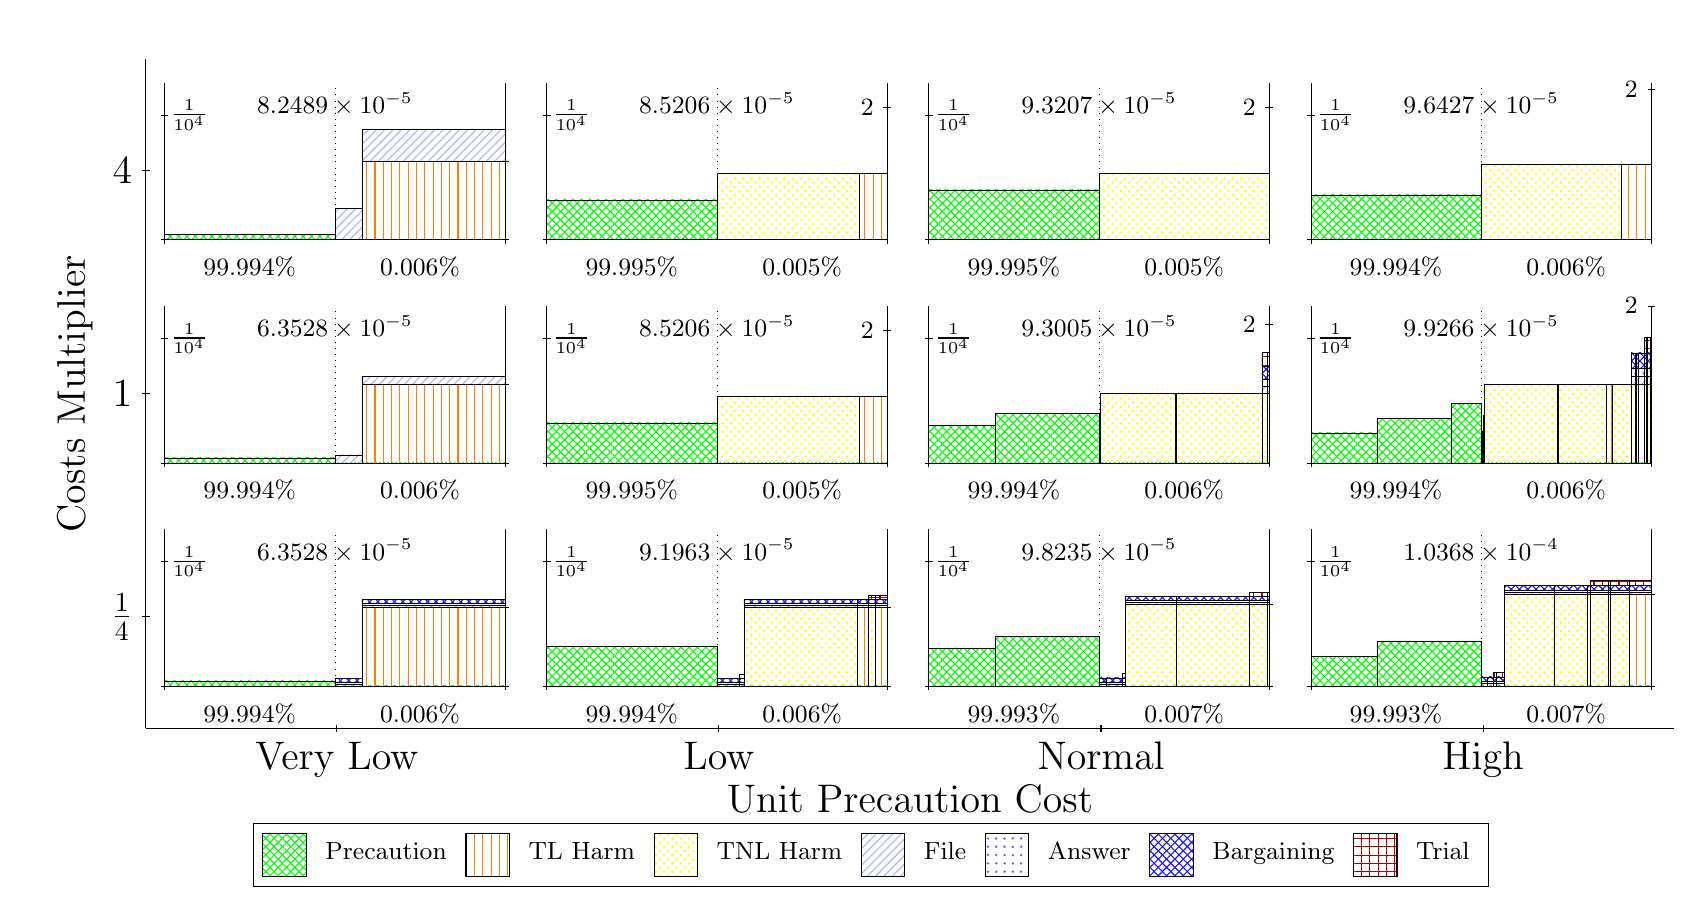
\begin{tikzpicture}
\clip(-0.5,-1.1) rectangle +(20.91,11);
\draw[black] (1,1) -- (1,9.5);
\node[rotate=90, fontscale=2, anchor=center] at (0.1, 5.25) {Costs Multiplier};
\draw[black] (0.95,2.4167) -- (1.05,2.4167);
\node[fontscale=2, anchor=east] at (0.95, 2.4167) {$\frac{1}{4}$};
\draw[black] (0.95,5.25) -- (1.05,5.25);
\node[fontscale=2, anchor=east] at (0.95, 5.25) {1};
\draw[black] (0.95,8.0833) -- (1.05,8.0833);
\node[fontscale=2, anchor=east] at (0.95, 8.0833) {4};

\draw[black] (1,1) -- (20.41,1);
\node[fontscale=2, anchor=center] at (10.705, 0.1) {Unit Precaution Cost};
\draw[black] (3.4263,0.95) -- (3.4263,1.05);
\node[fontscale=2, anchor=north] at (3.4263, 0.95) {Very Low};
\draw[black] (8.2788,0.95) -- (8.2788,1.05);
\node[fontscale=2, anchor=north] at (8.2788, 0.95) {Low};
\draw[black] (13.131,0.95) -- (13.131,1.05);
\node[fontscale=2, anchor=north] at (13.131, 0.95) {Normal};
\draw[black] (17.984,0.95) -- (17.984,1.05);
\node[fontscale=2, anchor=north] at (17.984, 0.95) {High};


\draw[pattern=crosshatch, pattern color=green,draw=black,very thin] (1.2381,1.54) rectangle (3.4013,1.6032);
\draw[pattern=crosshatch, pattern color=green,draw=black,very thin] (3.4013,1.54) rectangle (3.7435,1.54);
\draw[pattern=north east lines, pattern color=blue!30,draw=black,very thin] (3.4013,1.54) rectangle (3.7435,1.565);
\draw[pattern=dots,  pattern color=blue!60,draw=black,very thin] (3.4013,1.565) rectangle (3.7435,1.59);
\draw[pattern=crosshatch,      pattern color=blue!90,draw=black,very thin] (3.4013,1.59) rectangle (3.7435,1.64);
\draw[pattern=crosshatch, pattern color=green,draw=black,very thin] (3.7435,1.54) rectangle (5.5644,1.54);
\draw[pattern=vertical lines, pattern color=orange,draw=black,very thin] (3.7435,1.54) rectangle (5.5644,2.5395);
\draw[pattern=north east lines, pattern color=blue!30,draw=black,very thin] (3.7435,2.5395) rectangle (5.5644,2.5645);
\draw[pattern=dots,  pattern color=blue!60,draw=black,very thin] (3.7435,2.5645) rectangle (5.5644,2.5895);
\draw[pattern=crosshatch,      pattern color=blue!90,draw=black,very thin] (3.7435,2.5895) rectangle (5.5644,2.6394);
\node[font=\small,text=black,anchor=north] at (3.4013, 3.5333) {$6.3528\times 10^{-5}$};
\draw[black,very thin] (1.2381,1.54) -- (1.2381,3.5333);
\draw[black,very thin] (1.1881,1.54) -- (1.2881,1.54);
\node[font=\small,text=black, anchor=west] at (1.1881, 1.54) {};
\draw[black,very thin] (1.1881,3.1212) -- (1.2881,3.1212);
\node[font=\small,text=black, anchor=west] at (1.1881, 3.1212) {$\frac{1}{10^{4}}$};

\draw[black,dotted,very thin] (3.4013,1.5998) -- (3.4013,3.4735);
\draw[black,very thin] (5.5644,1.54) -- (5.5644,3.5333);
\draw[black,very thin] (5.5144,1.54) -- (5.6144,1.54);
\node[font=\small,text=black, anchor=east] at (5.5144, 1.54) {\contour{white}{}};
\draw[black,very thin] (5.5144,2.5395) -- (5.6144,2.5395);
\node[font=\small,text=black, anchor=east] at (5.5144, 2.5395) {\contour{white}{}};

\draw[black,very thin] (1.2381,1.54) -- (5.5644,1.54);
\draw[black,very thin] (1.2381,1.49) -- (1.2381,1.59);
\node[font=\small,text=black, anchor=north] at (1.2381, 1.49) {};
\draw[black,very thin] (5.5644,1.49) -- (5.5644,1.59);
\node[font=\small,text=black, anchor=north] at (5.5644, 1.49) {};

\node[font=\small,text=black,anchor=south] at (2.3197, 0.94) {99.994\%};
\node[font=\small,text=black,anchor=south] at (4.4828, 0.94) {0.006\%};

\draw[pattern=crosshatch, pattern color=green,draw=black,very thin] (6.0906,1.54) rectangle (8.2538,2.046);
\draw[pattern=crosshatch, pattern color=green,draw=black,very thin] (8.2538,1.54) rectangle (8.5357,1.54);
\draw[pattern=north east lines, pattern color=blue!30,draw=black,very thin] (8.2538,1.54) rectangle (8.5357,1.565);
\draw[pattern=dots,  pattern color=blue!60,draw=black,very thin] (8.2538,1.565) rectangle (8.5357,1.59);
\draw[pattern=crosshatch,      pattern color=blue!90,draw=black,very thin] (8.2538,1.59) rectangle (8.5357,1.64);
\draw[pattern=crosshatch, pattern color=green,draw=black,very thin] (8.5357,1.54) rectangle (8.596,1.54);
\draw[pattern=north east lines, pattern color=blue!30,draw=black,very thin] (8.5357,1.54) rectangle (8.596,1.565);
\draw[pattern=dots,  pattern color=blue!60,draw=black,very thin] (8.5357,1.565) rectangle (8.596,1.59);
\draw[pattern=crosshatch,      pattern color=blue!90,draw=black,very thin] (8.5357,1.59) rectangle (8.596,1.64);
\draw[pattern=grid,            pattern color=red!70!black,draw=black,very thin] (8.5357,1.64) rectangle (8.596,1.69);
\draw[pattern=crosshatch, pattern color=green,draw=black,very thin] (8.596,1.54) rectangle (10.04,1.54);
\draw[pattern=crosshatch dots, pattern color=yellow,draw=black,very thin] (8.596,1.54) rectangle (10.04,2.5395);
\draw[pattern=north east lines, pattern color=blue!30,draw=black,very thin] (8.596,2.5395) rectangle (10.04,2.5645);
\draw[pattern=dots,  pattern color=blue!60,draw=black,very thin] (8.596,2.5645) rectangle (10.04,2.5895);
\draw[pattern=crosshatch,      pattern color=blue!90,draw=black,very thin] (8.596,2.5895) rectangle (10.04,2.6395);
\draw[pattern=crosshatch, pattern color=green,draw=black,very thin] (10.04,1.54) rectangle (10.179,1.54);
\draw[pattern=vertical lines, pattern color=orange,draw=black,very thin] (10.04,1.54) rectangle (10.179,2.5395);
\draw[pattern=north east lines, pattern color=blue!30,draw=black,very thin] (10.04,2.5395) rectangle (10.179,2.5645);
\draw[pattern=dots,  pattern color=blue!60,draw=black,very thin] (10.04,2.5645) rectangle (10.179,2.5895);
\draw[pattern=crosshatch,      pattern color=blue!90,draw=black,very thin] (10.04,2.5895) rectangle (10.179,2.6395);
\draw[pattern=crosshatch, pattern color=green,draw=black,very thin] (10.179,1.54) rectangle (10.26,1.54);
\draw[pattern=crosshatch dots, pattern color=yellow,draw=black,very thin] (10.179,1.54) rectangle (10.26,2.5395);
\draw[pattern=north east lines, pattern color=blue!30,draw=black,very thin] (10.179,2.5395) rectangle (10.26,2.5645);
\draw[pattern=dots,  pattern color=blue!60,draw=black,very thin] (10.179,2.5645) rectangle (10.26,2.5895);
\draw[pattern=crosshatch,      pattern color=blue!90,draw=black,very thin] (10.179,2.5895) rectangle (10.26,2.6395);
\draw[pattern=grid,            pattern color=red!70!black,draw=black,very thin] (10.179,2.6395) rectangle (10.26,2.6894);
\draw[pattern=crosshatch, pattern color=green,draw=black,very thin] (10.26,1.54) rectangle (10.417,1.54);
\draw[pattern=vertical lines, pattern color=orange,draw=black,very thin] (10.26,1.54) rectangle (10.417,2.5395);
\draw[pattern=north east lines, pattern color=blue!30,draw=black,very thin] (10.26,2.5395) rectangle (10.417,2.5645);
\draw[pattern=dots,  pattern color=blue!60,draw=black,very thin] (10.26,2.5645) rectangle (10.417,2.5895);
\draw[pattern=crosshatch,      pattern color=blue!90,draw=black,very thin] (10.26,2.5895) rectangle (10.417,2.6395);
\draw[pattern=grid,            pattern color=red!70!black,draw=black,very thin] (10.26,2.6395) rectangle (10.417,2.6894);
\node[font=\small,text=black,anchor=north] at (8.2538, 3.5333) {$9.1963\times 10^{-5}$};
\draw[black,very thin] (6.0906,1.54) -- (6.0906,3.5333);
\draw[black,very thin] (6.0406,1.54) -- (6.1406,1.54);
\node[font=\small,text=black, anchor=west] at (6.0406, 1.54) {};
\draw[black,very thin] (6.0406,3.1212) -- (6.1406,3.1212);
\node[font=\small,text=black, anchor=west] at (6.0406, 3.1212) {$\frac{1}{10^{4}}$};

\draw[black,dotted,very thin] (8.2538,1.5998) -- (8.2538,3.4735);
\draw[black,very thin] (10.417,1.54) -- (10.417,3.5333);
\draw[black,very thin] (10.367,1.54) -- (10.467,1.54);
\node[font=\small,text=black, anchor=east] at (10.367, 1.54) {\contour{white}{}};
\draw[black,very thin] (10.367,2.5395) -- (10.467,2.5395);
\node[font=\small,text=black, anchor=east] at (10.367, 2.5395) {\contour{white}{}};

\draw[black,very thin] (6.0906,1.54) -- (10.417,1.54);
\draw[black,very thin] (6.0906,1.49) -- (6.0906,1.59);
\node[font=\small,text=black, anchor=north] at (6.0906, 1.49) {};
\draw[black,very thin] (10.417,1.49) -- (10.417,1.59);
\node[font=\small,text=black, anchor=north] at (10.417, 1.49) {};

\node[font=\small,text=black,anchor=south] at (7.1722, 0.94) {99.994\%};
\node[font=\small,text=black,anchor=south] at (9.3353, 0.94) {0.006\%};

\draw[pattern=crosshatch, pattern color=green,draw=black,very thin] (10.943,1.54) rectangle (11.791,2.0144);
\draw[pattern=crosshatch, pattern color=green,draw=black,very thin] (11.791,1.54) rectangle (13.106,2.1725);
\draw[pattern=crosshatch, pattern color=green,draw=black,very thin] (13.106,1.54) rectangle (13.197,1.54);
\draw[pattern=north east lines, pattern color=blue!30,draw=black,very thin] (13.106,1.54) rectangle (13.197,1.5658);
\draw[pattern=dots,  pattern color=blue!60,draw=black,very thin] (13.106,1.5658) rectangle (13.197,1.5916);
\draw[pattern=crosshatch,      pattern color=blue!90,draw=black,very thin] (13.106,1.5916) rectangle (13.197,1.6431);
\draw[pattern=crosshatch, pattern color=green,draw=black,very thin] (13.197,1.54) rectangle (13.398,1.54);
\draw[pattern=north east lines, pattern color=blue!30,draw=black,very thin] (13.197,1.54) rectangle (13.398,1.5658);
\draw[pattern=dots,  pattern color=blue!60,draw=black,very thin] (13.197,1.5658) rectangle (13.398,1.5916);
\draw[pattern=crosshatch,      pattern color=blue!90,draw=black,very thin] (13.197,1.5916) rectangle (13.398,1.6431);
\draw[pattern=crosshatch, pattern color=green,draw=black,very thin] (13.398,1.54) rectangle (13.438,1.54);
\draw[pattern=north east lines, pattern color=blue!30,draw=black,very thin] (13.398,1.54) rectangle (13.438,1.5658);
\draw[pattern=dots,  pattern color=blue!60,draw=black,very thin] (13.398,1.5658) rectangle (13.438,1.5916);
\draw[pattern=crosshatch,      pattern color=blue!90,draw=black,very thin] (13.398,1.5916) rectangle (13.438,1.6431);
\draw[pattern=grid,            pattern color=red!70!black,draw=black,very thin] (13.398,1.6431) rectangle (13.438,1.6947);
\draw[pattern=crosshatch, pattern color=green,draw=black,very thin] (13.438,1.54) rectangle (14.083,1.54);
\draw[pattern=crosshatch dots, pattern color=yellow,draw=black,very thin] (13.438,1.54) rectangle (14.083,2.5709);
\draw[pattern=north east lines, pattern color=blue!30,draw=black,very thin] (13.438,2.5709) rectangle (14.083,2.5967);
\draw[pattern=dots,  pattern color=blue!60,draw=black,very thin] (13.438,2.5967) rectangle (14.083,2.6225);
\draw[pattern=crosshatch,      pattern color=blue!90,draw=black,very thin] (13.438,2.6225) rectangle (14.083,2.674);
\draw[pattern=crosshatch, pattern color=green,draw=black,very thin] (14.083,1.54) rectangle (14.085,1.54);
\draw[pattern=vertical lines, pattern color=orange,draw=black,very thin] (14.083,1.54) rectangle (14.085,2.5709);
\draw[pattern=north east lines, pattern color=blue!30,draw=black,very thin] (14.083,2.5709) rectangle (14.085,2.5967);
\draw[pattern=dots,  pattern color=blue!60,draw=black,very thin] (14.083,2.5967) rectangle (14.085,2.6225);
\draw[pattern=crosshatch,      pattern color=blue!90,draw=black,very thin] (14.083,2.6225) rectangle (14.085,2.674);
\draw[pattern=crosshatch, pattern color=green,draw=black,very thin] (14.085,1.54) rectangle (15.016,1.54);
\draw[pattern=crosshatch dots, pattern color=yellow,draw=black,very thin] (14.085,1.54) rectangle (15.016,2.5709);
\draw[pattern=north east lines, pattern color=blue!30,draw=black,very thin] (14.085,2.5709) rectangle (15.016,2.5967);
\draw[pattern=dots,  pattern color=blue!60,draw=black,very thin] (14.085,2.5967) rectangle (15.016,2.6225);
\draw[pattern=crosshatch,      pattern color=blue!90,draw=black,very thin] (14.085,2.6225) rectangle (15.016,2.674);
\draw[pattern=crosshatch, pattern color=green,draw=black,very thin] (15.016,1.54) rectangle (15.241,1.54);
\draw[pattern=crosshatch dots, pattern color=yellow,draw=black,very thin] (15.016,1.54) rectangle (15.241,2.5709);
\draw[pattern=north east lines, pattern color=blue!30,draw=black,very thin] (15.016,2.5709) rectangle (15.241,2.5967);
\draw[pattern=dots,  pattern color=blue!60,draw=black,very thin] (15.016,2.5967) rectangle (15.241,2.6225);
\draw[pattern=crosshatch,      pattern color=blue!90,draw=black,very thin] (15.016,2.6225) rectangle (15.241,2.674);
\draw[pattern=grid,            pattern color=red!70!black,draw=black,very thin] (15.016,2.674) rectangle (15.241,2.7255);
\draw[pattern=crosshatch, pattern color=green,draw=black,very thin] (15.241,1.54) rectangle (15.269,1.54);
\draw[pattern=vertical lines, pattern color=orange,draw=black,very thin] (15.241,1.54) rectangle (15.269,2.5709);
\draw[pattern=north east lines, pattern color=blue!30,draw=black,very thin] (15.241,2.5709) rectangle (15.269,2.5967);
\draw[pattern=dots,  pattern color=blue!60,draw=black,very thin] (15.241,2.5967) rectangle (15.269,2.6225);
\draw[pattern=crosshatch,      pattern color=blue!90,draw=black,very thin] (15.241,2.6225) rectangle (15.269,2.674);
\draw[pattern=grid,            pattern color=red!70!black,draw=black,very thin] (15.241,2.674) rectangle (15.269,2.7255);
\node[font=\small,text=black,anchor=north] at (13.106, 3.5333) {$9.8235\times 10^{-5}$};
\draw[black,very thin] (10.943,1.54) -- (10.943,3.5333);
\draw[black,very thin] (10.893,1.54) -- (10.993,1.54);
\node[font=\small,text=black, anchor=west] at (10.893, 1.54) {};
\draw[black,very thin] (10.893,3.1212) -- (10.993,3.1212);
\node[font=\small,text=black, anchor=west] at (10.893, 3.1212) {$\frac{1}{10^{4}}$};

\draw[black,dotted,very thin] (13.106,1.5998) -- (13.106,3.4735);
\draw[black,very thin] (15.269,1.54) -- (15.269,3.5333);
\draw[black,very thin] (15.219,1.54) -- (15.319,1.54);
\node[font=\small,text=black, anchor=east] at (15.219, 1.54) {\contour{white}{}};
\draw[black,very thin] (15.219,2.5709) -- (15.319,2.5709);
\node[font=\small,text=black, anchor=east] at (15.219, 2.5709) {\contour{white}{}};

\draw[black,very thin] (10.943,1.54) -- (15.269,1.54);
\draw[black,very thin] (10.943,1.49) -- (10.943,1.59);
\node[font=\small,text=black, anchor=north] at (10.943, 1.49) {};
\draw[black,very thin] (15.269,1.49) -- (15.269,1.59);
\node[font=\small,text=black, anchor=north] at (15.269, 1.49) {};

\node[font=\small,text=black,anchor=south] at (12.025, 0.94) {99.993\%};
\node[font=\small,text=black,anchor=south] at (14.188, 0.94) {0.007\%};

\draw[pattern=crosshatch, pattern color=green,draw=black,very thin] (15.796,1.54) rectangle (16.643,1.9195);
\draw[pattern=crosshatch, pattern color=green,draw=black,very thin] (16.643,1.54) rectangle (17.959,2.1092);
\draw[pattern=crosshatch, pattern color=green,draw=black,very thin] (17.959,1.54) rectangle (18.039,1.54);
\draw[pattern=north east lines, pattern color=blue!30,draw=black,very thin] (17.959,1.54) rectangle (18.039,1.5691);
\draw[pattern=dots,  pattern color=blue!60,draw=black,very thin] (17.959,1.5691) rectangle (18.039,1.5981);
\draw[pattern=crosshatch,      pattern color=blue!90,draw=black,very thin] (17.959,1.5981) rectangle (18.039,1.6562);
\draw[pattern=crosshatch, pattern color=green,draw=black,very thin] (18.039,1.54) rectangle (18.115,1.54);
\draw[pattern=north east lines, pattern color=blue!30,draw=black,very thin] (18.039,1.54) rectangle (18.115,1.5691);
\draw[pattern=dots,  pattern color=blue!60,draw=black,very thin] (18.039,1.5691) rectangle (18.115,1.5981);
\draw[pattern=crosshatch,      pattern color=blue!90,draw=black,very thin] (18.039,1.5981) rectangle (18.115,1.6562);
\draw[pattern=crosshatch, pattern color=green,draw=black,very thin] (18.115,1.54) rectangle (18.15,1.54);
\draw[pattern=north east lines, pattern color=blue!30,draw=black,very thin] (18.115,1.54) rectangle (18.15,1.5691);
\draw[pattern=dots,  pattern color=blue!60,draw=black,very thin] (18.115,1.5691) rectangle (18.15,1.5981);
\draw[pattern=crosshatch,      pattern color=blue!90,draw=black,very thin] (18.115,1.5981) rectangle (18.15,1.6562);
\draw[pattern=grid,            pattern color=red!70!black,draw=black,very thin] (18.115,1.6562) rectangle (18.15,1.7143);
\draw[pattern=crosshatch, pattern color=green,draw=black,very thin] (18.15,1.54) rectangle (18.253,1.54);
\draw[pattern=north east lines, pattern color=blue!30,draw=black,very thin] (18.15,1.54) rectangle (18.253,1.5691);
\draw[pattern=dots,  pattern color=blue!60,draw=black,very thin] (18.15,1.5691) rectangle (18.253,1.5981);
\draw[pattern=crosshatch,      pattern color=blue!90,draw=black,very thin] (18.15,1.5981) rectangle (18.253,1.6562);
\draw[pattern=grid,            pattern color=red!70!black,draw=black,very thin] (18.15,1.6562) rectangle (18.253,1.7143);
\draw[pattern=crosshatch, pattern color=green,draw=black,very thin] (18.253,1.54) rectangle (18.883,1.54);
\draw[pattern=crosshatch dots, pattern color=yellow,draw=black,very thin] (18.253,1.54) rectangle (18.883,2.7018);
\draw[pattern=north east lines, pattern color=blue!30,draw=black,very thin] (18.253,2.7018) rectangle (18.883,2.7309);
\draw[pattern=dots,  pattern color=blue!60,draw=black,very thin] (18.253,2.7309) rectangle (18.883,2.7599);
\draw[pattern=crosshatch,      pattern color=blue!90,draw=black,very thin] (18.253,2.7599) rectangle (18.883,2.818);
\draw[pattern=crosshatch, pattern color=green,draw=black,very thin] (18.883,1.54) rectangle (18.884,1.54);
\draw[pattern=vertical lines, pattern color=orange,draw=black,very thin] (18.883,1.54) rectangle (18.884,2.7018);
\draw[pattern=north east lines, pattern color=blue!30,draw=black,very thin] (18.883,2.7018) rectangle (18.884,2.7309);
\draw[pattern=dots,  pattern color=blue!60,draw=black,very thin] (18.883,2.7309) rectangle (18.884,2.7599);
\draw[pattern=crosshatch,      pattern color=blue!90,draw=black,very thin] (18.883,2.7599) rectangle (18.884,2.818);
\draw[pattern=crosshatch, pattern color=green,draw=black,very thin] (18.884,1.54) rectangle (19.309,1.54);
\draw[pattern=crosshatch dots, pattern color=yellow,draw=black,very thin] (18.884,1.54) rectangle (19.309,2.7018);
\draw[pattern=north east lines, pattern color=blue!30,draw=black,very thin] (18.884,2.7018) rectangle (19.309,2.7309);
\draw[pattern=dots,  pattern color=blue!60,draw=black,very thin] (18.884,2.7309) rectangle (19.309,2.7599);
\draw[pattern=crosshatch,      pattern color=blue!90,draw=black,very thin] (18.884,2.7599) rectangle (19.309,2.818);
\draw[pattern=crosshatch, pattern color=green,draw=black,very thin] (19.309,1.54) rectangle (19.341,1.54);
\draw[pattern=vertical lines, pattern color=orange,draw=black,very thin] (19.309,1.54) rectangle (19.341,2.7018);
\draw[pattern=north east lines, pattern color=blue!30,draw=black,very thin] (19.309,2.7018) rectangle (19.341,2.7309);
\draw[pattern=dots,  pattern color=blue!60,draw=black,very thin] (19.309,2.7309) rectangle (19.341,2.7599);
\draw[pattern=crosshatch,      pattern color=blue!90,draw=black,very thin] (19.309,2.7599) rectangle (19.341,2.818);
\draw[pattern=crosshatch, pattern color=green,draw=black,very thin] (19.341,1.54) rectangle (19.57,1.54);
\draw[pattern=crosshatch dots, pattern color=yellow,draw=black,very thin] (19.341,1.54) rectangle (19.57,2.7018);
\draw[pattern=north east lines, pattern color=blue!30,draw=black,very thin] (19.341,2.7018) rectangle (19.57,2.7309);
\draw[pattern=dots,  pattern color=blue!60,draw=black,very thin] (19.341,2.7309) rectangle (19.57,2.7599);
\draw[pattern=crosshatch,      pattern color=blue!90,draw=black,very thin] (19.341,2.7599) rectangle (19.57,2.818);
\draw[pattern=grid,            pattern color=red!70!black,draw=black,very thin] (19.341,2.818) rectangle (19.57,2.8761);
\draw[pattern=crosshatch, pattern color=green,draw=black,very thin] (19.57,1.54) rectangle (19.598,1.54);
\draw[pattern=vertical lines, pattern color=orange,draw=black,very thin] (19.57,1.54) rectangle (19.598,2.7018);
\draw[pattern=north east lines, pattern color=blue!30,draw=black,very thin] (19.57,2.7018) rectangle (19.598,2.7309);
\draw[pattern=dots,  pattern color=blue!60,draw=black,very thin] (19.57,2.7309) rectangle (19.598,2.7599);
\draw[pattern=crosshatch,      pattern color=blue!90,draw=black,very thin] (19.57,2.7599) rectangle (19.598,2.818);
\draw[pattern=grid,            pattern color=red!70!black,draw=black,very thin] (19.57,2.818) rectangle (19.598,2.8761);
\draw[pattern=crosshatch, pattern color=green,draw=black,very thin] (19.598,1.54) rectangle (19.841,1.54);
\draw[pattern=crosshatch dots, pattern color=yellow,draw=black,very thin] (19.598,1.54) rectangle (19.841,2.7018);
\draw[pattern=north east lines, pattern color=blue!30,draw=black,very thin] (19.598,2.7018) rectangle (19.841,2.7309);
\draw[pattern=dots,  pattern color=blue!60,draw=black,very thin] (19.598,2.7309) rectangle (19.841,2.7599);
\draw[pattern=crosshatch,      pattern color=blue!90,draw=black,very thin] (19.598,2.7599) rectangle (19.841,2.818);
\draw[pattern=grid,            pattern color=red!70!black,draw=black,very thin] (19.598,2.818) rectangle (19.841,2.8761);
\draw[pattern=crosshatch, pattern color=green,draw=black,very thin] (19.841,1.54) rectangle (20.122,1.54);
\draw[pattern=vertical lines, pattern color=orange,draw=black,very thin] (19.841,1.54) rectangle (20.122,2.7018);
\draw[pattern=north east lines, pattern color=blue!30,draw=black,very thin] (19.841,2.7018) rectangle (20.122,2.7309);
\draw[pattern=dots,  pattern color=blue!60,draw=black,very thin] (19.841,2.7309) rectangle (20.122,2.7599);
\draw[pattern=crosshatch,      pattern color=blue!90,draw=black,very thin] (19.841,2.7599) rectangle (20.122,2.818);
\draw[pattern=grid,            pattern color=red!70!black,draw=black,very thin] (19.841,2.818) rectangle (20.122,2.8761);
\node[font=\small,text=black,anchor=north] at (17.959, 3.5333) {$1.0368\times 10^{-4}$};
\draw[black,very thin] (15.796,1.54) -- (15.796,3.5333);
\draw[black,very thin] (15.746,1.54) -- (15.846,1.54);
\node[font=\small,text=black, anchor=west] at (15.746, 1.54) {};
\draw[black,very thin] (15.746,3.1212) -- (15.846,3.1212);
\node[font=\small,text=black, anchor=west] at (15.746, 3.1212) {$\frac{1}{10^{4}}$};

\draw[black,dotted,very thin] (17.959,1.5998) -- (17.959,3.4735);
\draw[black,very thin] (20.122,1.54) -- (20.122,3.5333);
\draw[black,very thin] (20.072,1.54) -- (20.172,1.54);
\node[font=\small,text=black, anchor=east] at (20.072, 1.54) {\contour{white}{}};
\draw[black,very thin] (20.072,2.7018) -- (20.172,2.7018);
\node[font=\small,text=black, anchor=east] at (20.072, 2.7018) {\contour{white}{}};

\draw[black,very thin] (15.796,1.54) -- (20.122,1.54);
\draw[black,very thin] (15.796,1.49) -- (15.796,1.59);
\node[font=\small,text=black, anchor=north] at (15.796, 1.49) {};
\draw[black,very thin] (20.122,1.49) -- (20.122,1.59);
\node[font=\small,text=black, anchor=north] at (20.122, 1.49) {};

\node[font=\small,text=black,anchor=south] at (16.877, 0.94) {99.993\%};
\node[font=\small,text=black,anchor=south] at (19.04, 0.94) {0.007\%};

\draw[pattern=crosshatch, pattern color=green,draw=black,very thin] (1.2381,4.3733) rectangle (3.4013,4.4366);
\draw[pattern=crosshatch, pattern color=green,draw=black,very thin] (3.4013,4.3733) rectangle (3.7435,4.3733);
\draw[pattern=north east lines, pattern color=blue!30,draw=black,very thin] (3.4013,4.3733) rectangle (3.7435,4.4733);
\draw[pattern=crosshatch, pattern color=green,draw=black,very thin] (3.7435,4.3733) rectangle (5.5644,4.3733);
\draw[pattern=vertical lines, pattern color=orange,draw=black,very thin] (3.7435,4.3733) rectangle (5.5644,5.3728);
\draw[pattern=north east lines, pattern color=blue!30,draw=black,very thin] (3.7435,5.3728) rectangle (5.5644,5.4728);
\node[font=\small,text=black,anchor=north] at (3.4013, 6.3667) {$6.3528\times 10^{-5}$};
\draw[black,very thin] (1.2381,4.3733) -- (1.2381,6.3667);
\draw[black,very thin] (1.1881,4.3733) -- (1.2881,4.3733);
\node[font=\small,text=black, anchor=west] at (1.1881, 4.3733) {};
\draw[black,very thin] (1.1881,5.9545) -- (1.2881,5.9545);
\node[font=\small,text=black, anchor=west] at (1.1881, 5.9545) {$\frac{1}{10^{4}}$};

\draw[black,dotted,very thin] (3.4013,4.4331) -- (3.4013,6.3069);
\draw[black,very thin] (5.5644,4.3733) -- (5.5644,6.3667);
\draw[black,very thin] (5.5144,4.3733) -- (5.6144,4.3733);
\node[font=\small,text=black, anchor=east] at (5.5144, 4.3733) {\contour{white}{}};
\draw[black,very thin] (5.5144,5.3728) -- (5.6144,5.3728);
\node[font=\small,text=black, anchor=east] at (5.5144, 5.3728) {\contour{white}{}};

\draw[black,very thin] (1.2381,4.3733) -- (5.5644,4.3733);
\draw[black,very thin] (1.2381,4.3233) -- (1.2381,4.4233);
\node[font=\small,text=black, anchor=north] at (1.2381, 4.3233) {};
\draw[black,very thin] (5.5644,4.3233) -- (5.5644,4.4233);
\node[font=\small,text=black, anchor=north] at (5.5644, 4.3233) {};

\node[font=\small,text=black,anchor=south] at (2.3197, 3.7733) {99.994\%};
\node[font=\small,text=black,anchor=south] at (4.4828, 3.7733) {0.006\%};

\draw[pattern=crosshatch, pattern color=green,draw=black,very thin] (6.0906,4.3733) rectangle (8.2538,4.8793);
\draw[pattern=crosshatch, pattern color=green,draw=black,very thin] (8.2538,4.3733) rectangle (10.066,4.3734);
\draw[pattern=crosshatch dots, pattern color=yellow,draw=black,very thin] (8.2538,4.3734) rectangle (10.066,5.2147);
\draw[pattern=crosshatch, pattern color=green,draw=black,very thin] (10.066,4.3733) rectangle (10.417,4.3734);
\draw[pattern=vertical lines, pattern color=orange,draw=black,very thin] (10.066,4.3734) rectangle (10.417,5.2147);
\node[font=\small,text=black,anchor=north] at (8.2538, 6.3667) {$8.5206\times 10^{-5}$};
\draw[black,very thin] (6.0906,4.3733) -- (6.0906,6.3667);
\draw[black,very thin] (6.0406,4.3733) -- (6.1406,4.3733);
\node[font=\small,text=black, anchor=west] at (6.0406, 4.3733) {};
\draw[black,very thin] (6.0406,5.9545) -- (6.1406,5.9545);
\node[font=\small,text=black, anchor=west] at (6.0406, 5.9545) {$\frac{1}{10^{4}}$};

\draw[black,dotted,very thin] (8.2538,4.4331) -- (8.2538,6.3069);
\draw[black,very thin] (10.417,4.3733) -- (10.417,6.3667);
\draw[black,very thin] (10.367,6.056) -- (10.467,6.056);
\node[font=\small,text=black, anchor=east] at (10.367, 6.056) {\contour{white}{2}};

\draw[black,very thin] (6.0906,4.3733) -- (10.417,4.3733);
\draw[black,very thin] (6.0906,4.3233) -- (6.0906,4.4233);
\node[font=\small,text=black, anchor=north] at (6.0906, 4.3233) {};
\draw[black,very thin] (10.417,4.3233) -- (10.417,4.4233);
\node[font=\small,text=black, anchor=north] at (10.417, 4.3233) {};

\node[font=\small,text=black,anchor=south] at (7.1722, 3.7733) {99.995\%};
\node[font=\small,text=black,anchor=south] at (9.3353, 3.7733) {0.005\%};

\draw[pattern=crosshatch, pattern color=green,draw=black,very thin] (10.943,4.3733) rectangle (11.791,4.8477);
\draw[pattern=crosshatch, pattern color=green,draw=black,very thin] (11.791,4.3733) rectangle (13.106,5.0058);
\draw[pattern=crosshatch, pattern color=green,draw=black,very thin] (13.106,4.3733) rectangle (13.122,4.3734);
\draw[pattern=north east lines, pattern color=blue!30,draw=black,very thin] (13.106,4.3734) rectangle (13.122,4.4613);
\draw[pattern=dots,  pattern color=blue!60,draw=black,very thin] (13.106,4.4613) rectangle (13.122,4.5492);
\draw[pattern=crosshatch,      pattern color=blue!90,draw=black,very thin] (13.106,4.5492) rectangle (13.122,4.7251);
\draw[pattern=grid,            pattern color=red!70!black,draw=black,very thin] (13.106,4.7251) rectangle (13.122,4.9009);
\draw[pattern=crosshatch, pattern color=green,draw=black,very thin] (13.122,4.3733) rectangle (14.072,4.3734);
\draw[pattern=crosshatch dots, pattern color=yellow,draw=black,very thin] (13.122,4.3734) rectangle (14.072,5.2526);
\draw[pattern=crosshatch, pattern color=green,draw=black,very thin] (14.072,4.3733) rectangle (14.082,4.3734);
\draw[pattern=vertical lines, pattern color=orange,draw=black,very thin] (14.072,4.3734) rectangle (14.082,5.2526);
\draw[pattern=crosshatch, pattern color=green,draw=black,very thin] (14.082,4.3733) rectangle (15.173,4.3734);
\draw[pattern=crosshatch dots, pattern color=yellow,draw=black,very thin] (14.082,4.3734) rectangle (15.173,5.2526);
\draw[pattern=crosshatch, pattern color=green,draw=black,very thin] (15.173,4.3733) rectangle (15.244,4.3734);
\draw[pattern=crosshatch dots, pattern color=yellow,draw=black,very thin] (15.173,4.3734) rectangle (15.244,5.2526);
\draw[pattern=north east lines, pattern color=blue!30,draw=black,very thin] (15.173,5.2526) rectangle (15.244,5.3406);
\draw[pattern=dots,  pattern color=blue!60,draw=black,very thin] (15.173,5.3406) rectangle (15.244,5.4285);
\draw[pattern=crosshatch,      pattern color=blue!90,draw=black,very thin] (15.173,5.4285) rectangle (15.244,5.6043);
\draw[pattern=grid,            pattern color=red!70!black,draw=black,very thin] (15.173,5.6043) rectangle (15.244,5.7802);
\draw[pattern=crosshatch, pattern color=green,draw=black,very thin] (15.244,4.3733) rectangle (15.269,4.3734);
\draw[pattern=vertical lines, pattern color=orange,draw=black,very thin] (15.244,4.3734) rectangle (15.269,5.2526);
\draw[pattern=north east lines, pattern color=blue!30,draw=black,very thin] (15.244,5.2526) rectangle (15.269,5.3406);
\draw[pattern=dots,  pattern color=blue!60,draw=black,very thin] (15.244,5.3406) rectangle (15.269,5.4285);
\draw[pattern=crosshatch,      pattern color=blue!90,draw=black,very thin] (15.244,5.4285) rectangle (15.269,5.6043);
\draw[pattern=grid,            pattern color=red!70!black,draw=black,very thin] (15.244,5.6043) rectangle (15.269,5.7802);
\node[font=\small,text=black,anchor=north] at (13.106, 6.3667) {$9.3005\times 10^{-5}$};
\draw[black,very thin] (10.943,4.3733) -- (10.943,6.3667);
\draw[black,very thin] (10.893,4.3733) -- (10.993,4.3733);
\node[font=\small,text=black, anchor=west] at (10.893, 4.3733) {};
\draw[black,very thin] (10.893,5.9545) -- (10.993,5.9545);
\node[font=\small,text=black, anchor=west] at (10.893, 5.9545) {$\frac{1}{10^{4}}$};

\draw[black,dotted,very thin] (13.106,4.4331) -- (13.106,6.3069);
\draw[black,very thin] (15.269,4.3733) -- (15.269,6.3667);
\draw[black,very thin] (15.219,6.1319) -- (15.319,6.1319);
\node[font=\small,text=black, anchor=east] at (15.219, 6.1319) {\contour{white}{2}};

\draw[black,very thin] (10.943,4.3733) -- (15.269,4.3733);
\draw[black,very thin] (10.943,4.3233) -- (10.943,4.4233);
\node[font=\small,text=black, anchor=north] at (10.943, 4.3233) {};
\draw[black,very thin] (15.269,4.3233) -- (15.269,4.4233);
\node[font=\small,text=black, anchor=north] at (15.269, 4.3233) {};

\node[font=\small,text=black,anchor=south] at (12.025, 3.7733) {99.994\%};
\node[font=\small,text=black,anchor=south] at (14.188, 3.7733) {0.006\%};

\draw[pattern=crosshatch, pattern color=green,draw=black,very thin] (15.796,4.3733) rectangle (16.643,4.7528);
\draw[pattern=crosshatch, pattern color=green,draw=black,very thin] (16.643,4.3733) rectangle (17.578,4.9426);
\draw[pattern=crosshatch, pattern color=green,draw=black,very thin] (17.578,4.3733) rectangle (17.959,5.1323);
\draw[pattern=crosshatch, pattern color=green,draw=black,very thin] (17.959,4.3733) rectangle (17.967,4.3734);
\draw[pattern=north east lines, pattern color=blue!30,draw=black,very thin] (17.959,4.3734) rectangle (17.967,4.473);
\draw[pattern=dots,  pattern color=blue!60,draw=black,very thin] (17.959,4.473) rectangle (17.967,4.5727);
\draw[pattern=crosshatch,      pattern color=blue!90,draw=black,very thin] (17.959,4.5727) rectangle (17.967,4.772);
\draw[pattern=crosshatch, pattern color=green,draw=black,very thin] (17.967,4.3733) rectangle (17.989,4.3734);
\draw[pattern=north east lines, pattern color=blue!30,draw=black,very thin] (17.967,4.3734) rectangle (17.989,4.473);
\draw[pattern=dots,  pattern color=blue!60,draw=black,very thin] (17.967,4.473) rectangle (17.989,4.5727);
\draw[pattern=crosshatch,      pattern color=blue!90,draw=black,very thin] (17.967,4.5727) rectangle (17.989,4.772);
\draw[pattern=crosshatch, pattern color=green,draw=black,very thin] (17.989,4.3733) rectangle (17.995,4.3734);
\draw[pattern=north east lines, pattern color=blue!30,draw=black,very thin] (17.989,4.3734) rectangle (17.995,4.473);
\draw[pattern=dots,  pattern color=blue!60,draw=black,very thin] (17.989,4.473) rectangle (17.995,4.5727);
\draw[pattern=crosshatch,      pattern color=blue!90,draw=black,very thin] (17.989,4.5727) rectangle (17.995,4.772);
\draw[pattern=grid,            pattern color=red!70!black,draw=black,very thin] (17.989,4.772) rectangle (17.995,4.9713);
\draw[pattern=crosshatch, pattern color=green,draw=black,very thin] (17.995,4.3733) rectangle (18.004,4.3734);
\draw[pattern=north east lines, pattern color=blue!30,draw=black,very thin] (17.995,4.3734) rectangle (18.004,4.473);
\draw[pattern=dots,  pattern color=blue!60,draw=black,very thin] (17.995,4.473) rectangle (18.004,4.5727);
\draw[pattern=crosshatch,      pattern color=blue!90,draw=black,very thin] (17.995,4.5727) rectangle (18.004,4.772);
\draw[pattern=grid,            pattern color=red!70!black,draw=black,very thin] (17.995,4.772) rectangle (18.004,4.9714);
\draw[pattern=crosshatch, pattern color=green,draw=black,very thin] (18.004,4.3733) rectangle (18.931,4.3734);
\draw[pattern=crosshatch dots, pattern color=yellow,draw=black,very thin] (18.004,4.3734) rectangle (18.931,5.37);
\draw[pattern=crosshatch, pattern color=green,draw=black,very thin] (18.931,4.3733) rectangle (18.94,4.3734);
\draw[pattern=vertical lines, pattern color=orange,draw=black,very thin] (18.931,4.3734) rectangle (18.94,5.37);
\draw[pattern=crosshatch, pattern color=green,draw=black,very thin] (18.94,4.3733) rectangle (19.55,4.3734);
\draw[pattern=crosshatch dots, pattern color=yellow,draw=black,very thin] (18.94,4.3734) rectangle (19.55,5.37);
\draw[pattern=crosshatch, pattern color=green,draw=black,very thin] (19.55,4.3733) rectangle (19.627,4.3734);
\draw[pattern=vertical lines, pattern color=orange,draw=black,very thin] (19.55,4.3734) rectangle (19.627,5.37);
\draw[pattern=crosshatch, pattern color=green,draw=black,very thin] (19.627,4.3733) rectangle (19.865,4.3734);
\draw[pattern=crosshatch dots, pattern color=yellow,draw=black,very thin] (19.627,4.3734) rectangle (19.865,5.37);
\draw[pattern=crosshatch, pattern color=green,draw=black,very thin] (19.865,4.3733) rectangle (19.91,4.3734);
\draw[pattern=crosshatch dots, pattern color=yellow,draw=black,very thin] (19.865,4.3734) rectangle (19.91,5.37);
\draw[pattern=north east lines, pattern color=blue!30,draw=black,very thin] (19.865,5.37) rectangle (19.91,5.4697);
\draw[pattern=dots,  pattern color=blue!60,draw=black,very thin] (19.865,5.4697) rectangle (19.91,5.5693);
\draw[pattern=crosshatch,      pattern color=blue!90,draw=black,very thin] (19.865,5.5693) rectangle (19.91,5.7687);
\draw[pattern=crosshatch, pattern color=green,draw=black,very thin] (19.91,4.3733) rectangle (19.923,4.3734);
\draw[pattern=vertical lines, pattern color=orange,draw=black,very thin] (19.91,4.3734) rectangle (19.923,5.37);
\draw[pattern=north east lines, pattern color=blue!30,draw=black,very thin] (19.91,5.37) rectangle (19.923,5.4697);
\draw[pattern=dots,  pattern color=blue!60,draw=black,very thin] (19.91,5.4697) rectangle (19.923,5.5693);
\draw[pattern=crosshatch,      pattern color=blue!90,draw=black,very thin] (19.91,5.5693) rectangle (19.923,5.7687);
\draw[pattern=crosshatch, pattern color=green,draw=black,very thin] (19.923,4.3733) rectangle (19.959,4.3734);
\draw[pattern=crosshatch dots, pattern color=yellow,draw=black,very thin] (19.923,4.3734) rectangle (19.959,5.37);
\draw[pattern=north east lines, pattern color=blue!30,draw=black,very thin] (19.923,5.37) rectangle (19.959,5.4697);
\draw[pattern=dots,  pattern color=blue!60,draw=black,very thin] (19.923,5.4697) rectangle (19.959,5.5693);
\draw[pattern=crosshatch,      pattern color=blue!90,draw=black,very thin] (19.923,5.5693) rectangle (19.959,5.7687);
\draw[pattern=crosshatch, pattern color=green,draw=black,very thin] (19.959,4.3733) rectangle (20.03,4.3734);
\draw[pattern=vertical lines, pattern color=orange,draw=black,very thin] (19.959,4.3734) rectangle (20.03,5.37);
\draw[pattern=north east lines, pattern color=blue!30,draw=black,very thin] (19.959,5.37) rectangle (20.03,5.4697);
\draw[pattern=dots,  pattern color=blue!60,draw=black,very thin] (19.959,5.4697) rectangle (20.03,5.5693);
\draw[pattern=crosshatch,      pattern color=blue!90,draw=black,very thin] (19.959,5.5693) rectangle (20.03,5.7687);
\draw[pattern=crosshatch, pattern color=green,draw=black,very thin] (20.03,4.3733) rectangle (20.06,4.3734);
\draw[pattern=crosshatch dots, pattern color=yellow,draw=black,very thin] (20.03,4.3734) rectangle (20.06,5.37);
\draw[pattern=north east lines, pattern color=blue!30,draw=black,very thin] (20.03,5.37) rectangle (20.06,5.4697);
\draw[pattern=dots,  pattern color=blue!60,draw=black,very thin] (20.03,5.4697) rectangle (20.06,5.5693);
\draw[pattern=crosshatch,      pattern color=blue!90,draw=black,very thin] (20.03,5.5693) rectangle (20.06,5.7687);
\draw[pattern=grid,            pattern color=red!70!black,draw=black,very thin] (20.03,5.7687) rectangle (20.06,5.968);
\draw[pattern=crosshatch, pattern color=green,draw=black,very thin] (20.06,4.3733) rectangle (20.071,4.3734);
\draw[pattern=vertical lines, pattern color=orange,draw=black,very thin] (20.06,4.3734) rectangle (20.071,5.37);
\draw[pattern=north east lines, pattern color=blue!30,draw=black,very thin] (20.06,5.37) rectangle (20.071,5.4697);
\draw[pattern=dots,  pattern color=blue!60,draw=black,very thin] (20.06,5.4697) rectangle (20.071,5.5693);
\draw[pattern=crosshatch,      pattern color=blue!90,draw=black,very thin] (20.06,5.5693) rectangle (20.071,5.7687);
\draw[pattern=grid,            pattern color=red!70!black,draw=black,very thin] (20.06,5.7687) rectangle (20.071,5.968);
\draw[pattern=crosshatch, pattern color=green,draw=black,very thin] (20.071,4.3733) rectangle (20.103,4.3734);
\draw[pattern=crosshatch dots, pattern color=yellow,draw=black,very thin] (20.071,4.3734) rectangle (20.103,5.37);
\draw[pattern=north east lines, pattern color=blue!30,draw=black,very thin] (20.071,5.37) rectangle (20.103,5.4697);
\draw[pattern=dots,  pattern color=blue!60,draw=black,very thin] (20.071,5.4697) rectangle (20.103,5.5693);
\draw[pattern=crosshatch,      pattern color=blue!90,draw=black,very thin] (20.071,5.5693) rectangle (20.103,5.7687);
\draw[pattern=grid,            pattern color=red!70!black,draw=black,very thin] (20.071,5.7687) rectangle (20.103,5.968);
\draw[pattern=crosshatch, pattern color=green,draw=black,very thin] (20.103,4.3733) rectangle (20.122,4.3734);
\draw[pattern=vertical lines, pattern color=orange,draw=black,very thin] (20.103,4.3734) rectangle (20.122,5.37);
\draw[pattern=north east lines, pattern color=blue!30,draw=black,very thin] (20.103,5.37) rectangle (20.122,5.4697);
\draw[pattern=dots,  pattern color=blue!60,draw=black,very thin] (20.103,5.4697) rectangle (20.122,5.5693);
\draw[pattern=crosshatch,      pattern color=blue!90,draw=black,very thin] (20.103,5.5693) rectangle (20.122,5.7687);
\draw[pattern=grid,            pattern color=red!70!black,draw=black,very thin] (20.103,5.7687) rectangle (20.122,5.968);
\node[font=\small,text=black,anchor=north] at (17.959, 6.3667) {$9.9266\times 10^{-5}$};
\draw[black,very thin] (15.796,4.3733) -- (15.796,6.3667);
\draw[black,very thin] (15.746,4.3733) -- (15.846,4.3733);
\node[font=\small,text=black, anchor=west] at (15.746, 4.3733) {};
\draw[black,very thin] (15.746,5.9545) -- (15.846,5.9545);
\node[font=\small,text=black, anchor=west] at (15.746, 5.9545) {$\frac{1}{10^{4}}$};

\draw[black,dotted,very thin] (17.959,4.4331) -- (17.959,6.3069);
\draw[black,very thin] (20.122,4.3733) -- (20.122,6.3667);
\draw[black,very thin] (20.072,6.3666) -- (20.172,6.3666);
\node[font=\small,text=black, anchor=east] at (20.072, 6.3666) {\contour{white}{2}};

\draw[black,very thin] (15.796,4.3733) -- (20.122,4.3733);
\draw[black,very thin] (15.796,4.3233) -- (15.796,4.4233);
\node[font=\small,text=black, anchor=north] at (15.796, 4.3233) {};
\draw[black,very thin] (20.122,4.3233) -- (20.122,4.4233);
\node[font=\small,text=black, anchor=north] at (20.122, 4.3233) {};

\node[font=\small,text=black,anchor=south] at (16.877, 3.7733) {99.994\%};
\node[font=\small,text=black,anchor=south] at (19.04, 3.7733) {0.006\%};

\draw[pattern=crosshatch, pattern color=green,draw=black,very thin] (1.2381,7.2067) rectangle (3.4013,7.2699);
\draw[pattern=crosshatch, pattern color=green,draw=black,very thin] (3.4013,7.2067) rectangle (3.7435,7.2067);
\draw[pattern=north east lines, pattern color=blue!30,draw=black,very thin] (3.4013,7.2067) rectangle (3.7435,7.6065);
\draw[pattern=crosshatch, pattern color=green,draw=black,very thin] (3.7435,7.2067) rectangle (5.5644,7.2067);
\draw[pattern=vertical lines, pattern color=orange,draw=black,very thin] (3.7435,7.2067) rectangle (5.5644,8.2061);
\draw[pattern=north east lines, pattern color=blue!30,draw=black,very thin] (3.7435,8.2061) rectangle (5.5644,8.6059);
\node[font=\small,text=black,anchor=north] at (3.4013, 9.2) {$8.2489\times 10^{-5}$};
\draw[black,very thin] (1.2381,7.2067) -- (1.2381,9.2);
\draw[black,very thin] (1.1881,7.2067) -- (1.2881,7.2067);
\node[font=\small,text=black, anchor=west] at (1.1881, 7.2067) {};
\draw[black,very thin] (1.1881,8.7879) -- (1.2881,8.7879);
\node[font=\small,text=black, anchor=west] at (1.1881, 8.7879) {$\frac{1}{10^{4}}$};

\draw[black,dotted,very thin] (3.4013,7.2665) -- (3.4013,9.1402);
\draw[black,very thin] (5.5644,7.2067) -- (5.5644,9.2);
\draw[black,very thin] (5.5144,7.2067) -- (5.6144,7.2067);
\node[font=\small,text=black, anchor=east] at (5.5144, 7.2067) {\contour{white}{}};
\draw[black,very thin] (5.5144,8.2061) -- (5.6144,8.2061);
\node[font=\small,text=black, anchor=east] at (5.5144, 8.2061) {\contour{white}{}};

\draw[black,very thin] (1.2381,7.2067) -- (5.5644,7.2067);
\draw[black,very thin] (1.2381,7.1567) -- (1.2381,7.2567);
\node[font=\small,text=black, anchor=north] at (1.2381, 7.1567) {};
\draw[black,very thin] (5.5644,7.1567) -- (5.5644,7.2567);
\node[font=\small,text=black, anchor=north] at (5.5644, 7.1567) {};

\node[font=\small,text=black,anchor=south] at (2.3197, 6.6067) {99.994\%};
\node[font=\small,text=black,anchor=south] at (4.4828, 6.6067) {0.006\%};

\draw[pattern=crosshatch, pattern color=green,draw=black,very thin] (6.0906,7.2067) rectangle (8.2538,7.7127);
\draw[pattern=crosshatch, pattern color=green,draw=black,very thin] (8.2538,7.2067) rectangle (10.066,7.2067);
\draw[pattern=crosshatch dots, pattern color=yellow,draw=black,very thin] (8.2538,7.2067) rectangle (10.066,8.048);
\draw[pattern=crosshatch, pattern color=green,draw=black,very thin] (10.066,7.2067) rectangle (10.417,7.2067);
\draw[pattern=vertical lines, pattern color=orange,draw=black,very thin] (10.066,7.2067) rectangle (10.417,8.048);
\node[font=\small,text=black,anchor=north] at (8.2538, 9.2) {$8.5206\times 10^{-5}$};
\draw[black,very thin] (6.0906,7.2067) -- (6.0906,9.2);
\draw[black,very thin] (6.0406,7.2067) -- (6.1406,7.2067);
\node[font=\small,text=black, anchor=west] at (6.0406, 7.2067) {};
\draw[black,very thin] (6.0406,8.7879) -- (6.1406,8.7879);
\node[font=\small,text=black, anchor=west] at (6.0406, 8.7879) {$\frac{1}{10^{4}}$};

\draw[black,dotted,very thin] (8.2538,7.2665) -- (8.2538,9.1402);
\draw[black,very thin] (10.417,7.2067) -- (10.417,9.2);
\draw[black,very thin] (10.367,8.8894) -- (10.467,8.8894);
\node[font=\small,text=black, anchor=east] at (10.367, 8.8894) {\contour{white}{2}};

\draw[black,very thin] (6.0906,7.2067) -- (10.417,7.2067);
\draw[black,very thin] (6.0906,7.1567) -- (6.0906,7.2567);
\node[font=\small,text=black, anchor=north] at (6.0906, 7.1567) {};
\draw[black,very thin] (10.417,7.1567) -- (10.417,7.2567);
\node[font=\small,text=black, anchor=north] at (10.417, 7.1567) {};

\node[font=\small,text=black,anchor=south] at (7.1722, 6.6067) {99.995\%};
\node[font=\small,text=black,anchor=south] at (9.3353, 6.6067) {0.005\%};

\draw[pattern=crosshatch, pattern color=green,draw=black,very thin] (10.943,7.2067) rectangle (13.106,7.8392);
\draw[pattern=crosshatch, pattern color=green,draw=black,very thin] (13.106,7.2067) rectangle (15.269,7.2067);
\draw[pattern=crosshatch dots, pattern color=yellow,draw=black,very thin] (13.106,7.2067) rectangle (15.269,8.0481);
\node[font=\small,text=black,anchor=north] at (13.106, 9.2) {$9.3207\times 10^{-5}$};
\draw[black,very thin] (10.943,7.2067) -- (10.943,9.2);
\draw[black,very thin] (10.893,7.2067) -- (10.993,7.2067);
\node[font=\small,text=black, anchor=west] at (10.893, 7.2067) {};
\draw[black,very thin] (10.893,8.7879) -- (10.993,8.7879);
\node[font=\small,text=black, anchor=west] at (10.893, 8.7879) {$\frac{1}{10^{4}}$};

\draw[black,dotted,very thin] (13.106,7.2665) -- (13.106,9.1402);
\draw[black,very thin] (15.269,7.2067) -- (15.269,9.2);
\draw[black,very thin] (15.219,8.8894) -- (15.319,8.8894);
\node[font=\small,text=black, anchor=east] at (15.219, 8.8894) {\contour{white}{2}};

\draw[black,very thin] (10.943,7.2067) -- (15.269,7.2067);
\draw[black,very thin] (10.943,7.1567) -- (10.943,7.2567);
\node[font=\small,text=black, anchor=north] at (10.943, 7.1567) {};
\draw[black,very thin] (15.269,7.1567) -- (15.269,7.2567);
\node[font=\small,text=black, anchor=north] at (15.269, 7.1567) {};

\node[font=\small,text=black,anchor=south] at (12.025, 6.6067) {99.995\%};
\node[font=\small,text=black,anchor=south] at (14.188, 6.6067) {0.005\%};

\draw[pattern=crosshatch, pattern color=green,draw=black,very thin] (15.796,7.2067) rectangle (17.959,7.7759);
\draw[pattern=crosshatch, pattern color=green,draw=black,very thin] (17.959,7.2067) rectangle (19.738,7.2067);
\draw[pattern=crosshatch dots, pattern color=yellow,draw=black,very thin] (17.959,7.2067) rectangle (19.738,8.1622);
\draw[pattern=crosshatch, pattern color=green,draw=black,very thin] (19.738,7.2067) rectangle (20.122,7.2067);
\draw[pattern=vertical lines, pattern color=orange,draw=black,very thin] (19.738,7.2067) rectangle (20.122,8.1622);
\node[font=\small,text=black,anchor=north] at (17.959, 9.2) {$9.6427\times 10^{-5}$};
\draw[black,very thin] (15.796,7.2067) -- (15.796,9.2);
\draw[black,very thin] (15.746,7.2067) -- (15.846,7.2067);
\node[font=\small,text=black, anchor=west] at (15.746, 7.2067) {};
\draw[black,very thin] (15.746,8.7879) -- (15.846,8.7879);
\node[font=\small,text=black, anchor=west] at (15.746, 8.7879) {$\frac{1}{10^{4}}$};

\draw[black,dotted,very thin] (17.959,7.2665) -- (17.959,9.1402);
\draw[black,very thin] (20.122,7.2067) -- (20.122,9.2);
\draw[black,very thin] (20.072,9.1177) -- (20.172,9.1177);
\node[font=\small,text=black, anchor=east] at (20.072, 9.1177) {\contour{white}{2}};

\draw[black,very thin] (15.796,7.2067) -- (20.122,7.2067);
\draw[black,very thin] (15.796,7.1567) -- (15.796,7.2567);
\node[font=\small,text=black, anchor=north] at (15.796, 7.1567) {};
\draw[black,very thin] (20.122,7.1567) -- (20.122,7.2567);
\node[font=\small,text=black, anchor=north] at (20.122, 7.1567) {};

\node[font=\small,text=black,anchor=south] at (16.877, 6.6067) {99.994\%};
\node[font=\small,text=black,anchor=south] at (19.04, 6.6067) {0.006\%};

\coordinate (LegendAnchor) at (10.205000000000002,0);
\begin{scope}[align=center]
\matrix[scale=0.6,draw=black,below=0.2cm of LegendAnchor,nodes={draw},column sep=0.12cm]{
\node[rectangle,draw,minimum width=0.55cm,minimum height=0.55cm,pattern=crosshatch, pattern color=green]{}; &
        \node[draw=none,font=\small]{Precaution}; &
\node[rectangle,draw,minimum width=0.55cm,minimum height=0.55cm,pattern=vertical lines, pattern color=orange]{}; &
        \node[draw=none,font=\small]{TL Harm}; &
\node[rectangle,draw,minimum width=0.55cm,minimum height=0.55cm,pattern=crosshatch dots, pattern color=yellow]{}; &
        \node[draw=none,font=\small]{TNL Harm}; &
\node[rectangle,draw,minimum width=0.55cm,minimum height=0.55cm,pattern=north east lines, pattern color=blue!30]{}; &
        \node[draw=none,font=\small]{File}; &
\node[rectangle,draw,minimum width=0.55cm,minimum height=0.55cm,pattern=dots, pattern color=blue!60]{}; &
        \node[draw=none,font=\small]{Answer}; &
\node[rectangle,draw,minimum width=0.55cm,minimum height=0.55cm,pattern=crosshatch, pattern color=blue!90]{}; &
        \node[draw=none,font=\small]{Bargaining}; &
\node[rectangle,draw,minimum width=0.55cm,minimum height=0.55cm,pattern=grid, pattern color=red!70!black]{}; &
        \node[draw=none,font=\small]{Trial}; \\
};\end{scope}

\end{tikzpicture}
\end{document}